
\chapter{Real-time video detection}
\label{chap:rltm}

real time -> 25fps
this is related work
% \section{Optimizing Video Object Detection via a Scale-Time Lattice}
% \section{Use of Detection networks for video processing}

\section{Detection networks}
\subsection{YOLO (2016)}
Following a success of neural network detectors from \textit{R-CNN} family. \citeauthor{bib:yolo} \cite{bib:yolo} introduced a new approach to object detection. \textit{You Only Look Once} is a CNN willing to sacrifice some precision with the goal of reaching real-time performance. 

It improves on the concept of \textit{R-CNN} type of networks by performing both classification and localization in single evaluation. This means that the \textit{YOLO} is much simpler single network that can be trained directly end-to-end. Thanks to straightforward architecture with single pass, \textit{YOLO} claims to run at 45fps on \textit{Titan X GPU}. \textit{YOLO} has better precision than other real-time detectors of its time, but it lacks the precision of slower models like \textit{Faster R-CNN}.

\begin{figure}
    \centering
    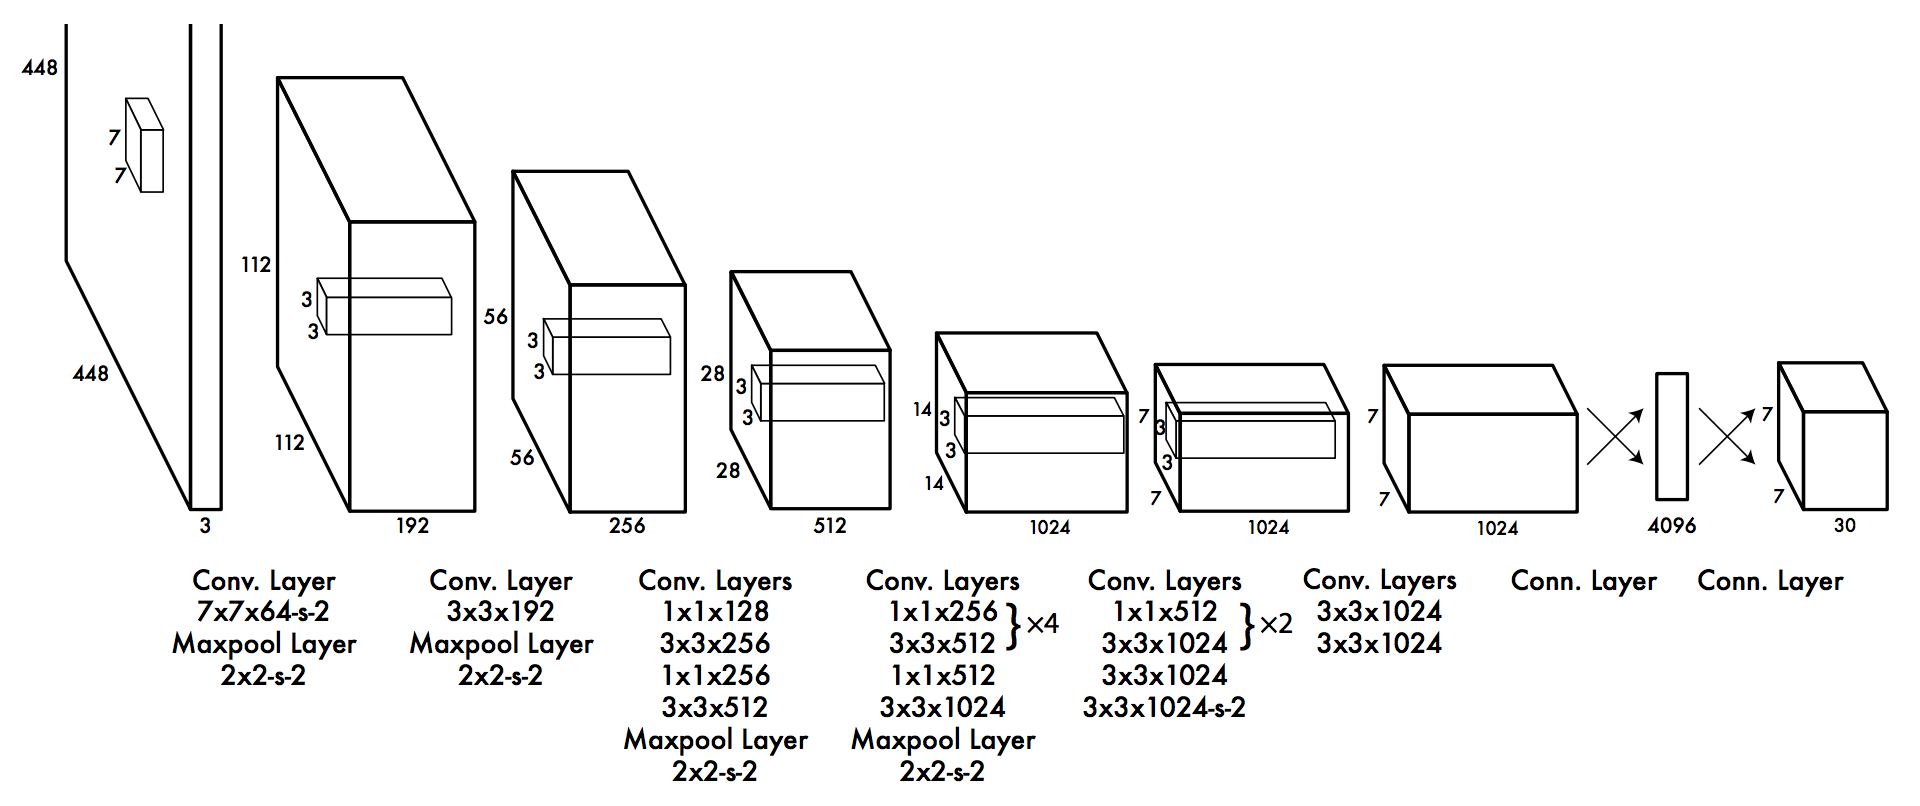
\includegraphics[width=\textwidth]{img/yoylo}
    \caption{\textit{YOLO} architecture for evaluating \textit{PASCAL VOC}. It uses 7 by 7 grid with 2 bboxes per cell. Detecting 20 categories, the output's shape is 7\x7\x30. From \cite[fig. 3]{bib:yolo}.}
    \label{fig:yolo} 
\end{figure}

\subsubsection{Detection}
Prediction in \textit{YOLO} work in a grid-based system. Image is divided into S\x S grid with a cell responsible for detecting the object centered in that cell. For each cell, \textit{YOLO} outputs class confidence predictions and five parameters for \textit{B} bboxes. Class confidence prediction represents conditional probability of said class, given the presence of the object in that cell. Classes are predicted for cells independently on number of bboxes. Each bounding box is given a confidence value that reflect IoU with ground-truth box. Other four parameters of bbox are it's center relative to the grid, and width and height relative to whole image. Bbox with higher confidence is chosen from cell and combined with most probable class. Final confidence of detected object is the product of those two values. We can see the illustration of this process on \cref{fig:yoloDet}.


\begin{figure}
    \centering
    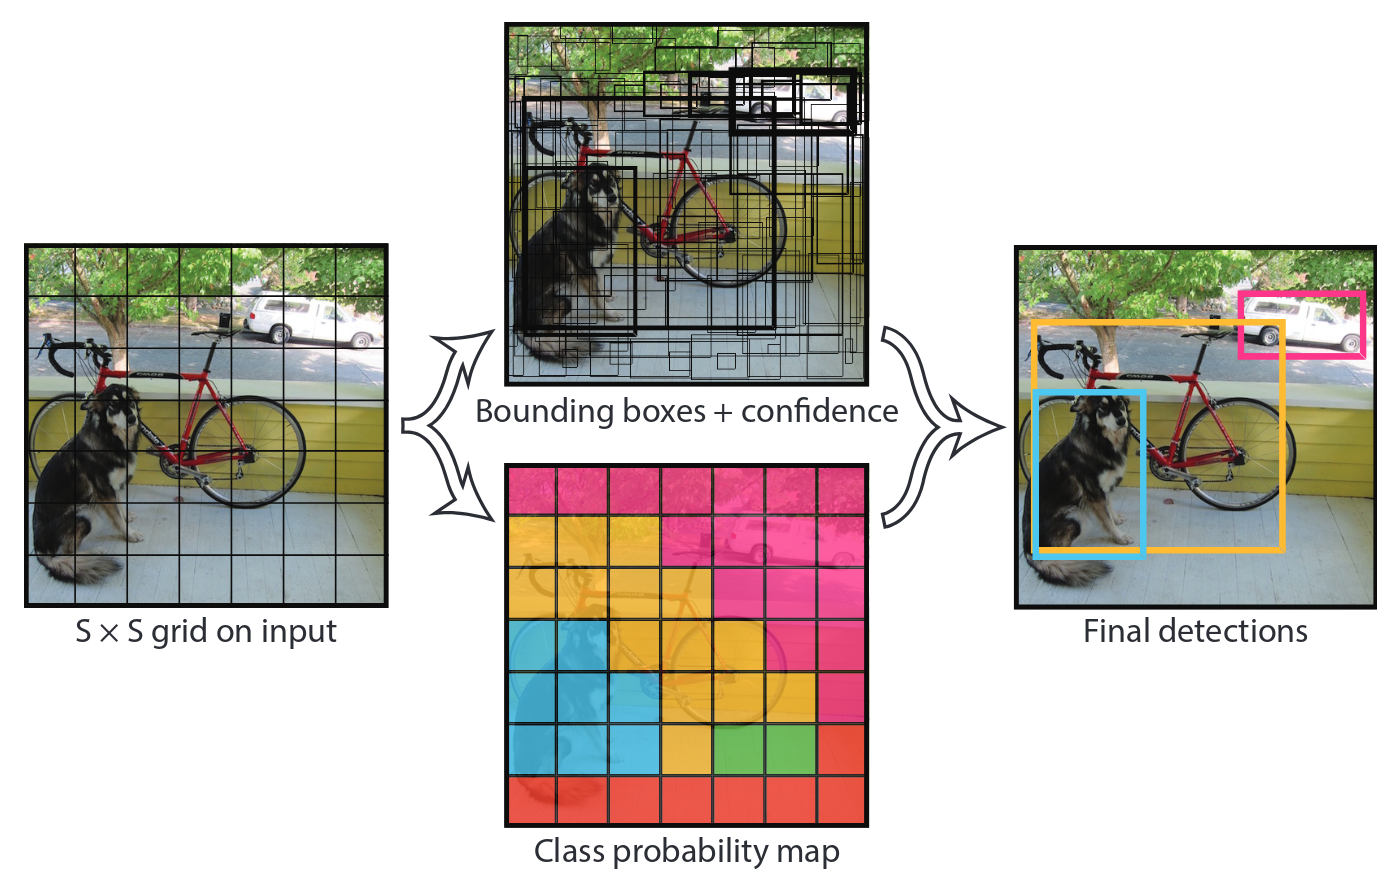
\includegraphics[width=\textwidth]{img/yoloDet}
    \caption{Detection process of \textit{YOLO}. From \cite[fig. 2]{bib:yolo}.}
    \label{fig:yoloDet} 
\end{figure}


\subsubsection{Architecture} 
\textit{YOLO} is designed as a single network that takes the input image and outputs bbox and class predictions. A design of the network is inspired by \textit{Inception} classification network. It uses 24 convolutional layers followed by 2 fully connected layers. Although it does not use inception modules, it relies on the 1\x1 reduction layers to speed up 3\x3 convolutions. Full architecture is shown on \cref{fig:yolo}. There is also a smaller and faster version, \textit{Fast YOLO}, with similar architecture but only 9 convolutional layers. Another possibility is to replace \textit{YOLO's} custom architecture with a feature extractor from a classification network. \textit{YOLO VGG-16} achieves better precision but sacrifices half of frames per second.

\subsection{Training}
First, convolutional layers are pretrained on the \textit{ImageNet} dataset, then the detection layers are added and whole network is trained for detection. The model is optimized using sum-squared error between predictions and ground-truths. The loss function is a sum of three parts, classification loss, localization loss, and bbox confidence loss. 

\paragraph{Classification loss}
\begin{align*}
\mathbf{CLS} = \sum_{i=0}^{S^2}\mathbbm{1}_i^{\text{obj}} \sum_{c\in \text{class}} (p_i(c) - \hat{p}_i(c))^2
\end{align*}

\paragraph{Localization loss}
\begin{align*}
\mathbf{LOC} &= \lambda_{\text{coord}} \sum_{i=0}^{S^2} \sum_{j=0}^B \mathbbm{1}_{ij}^{\text{obj}} \left[(x_i - \hat{x}_i)^2 + (y_i - \hat{y}_i)^2\right] \\
 &+  \lambda_{\text{coord}} \sum_{i=0}^{S^2} \sum_{j=0}^B \mathbbm{1}_{ij}^{\text{obj}} \left[(\sqrt{w_i} - \sqrt{\hat{w}_i})^2 + (\sqrt{h_i} - \sqrt{\hat{h}_i)^2}\right]
\end{align*}

\paragraph{Confidence loss}
\begin{align*}
\mathbf{CNF} &= \sum_{i=0}^{S^2} \sum_{j=0}^B \mathbbm{1}_{ij}^{\text{obj}} (C_i - \hat{C}_i)^2 
+ \lambda_{\text{noobj}} \sum_{i=0}^{S^2} \sum_{j=0}^B \mathbbm{1}_{ij}^{\text{noobj}} (C_i - \hat{C}_i)^2
\end{align*}

\noindent where $\mathbbm{1}^{\text{obj}}_i$ denotes if object appears in cell $i$ and $\mathbbm{1}^{\text{obj}}_{ij}$ denotes that the $j$th bounding box predictor in cell $i$ is responsible for that prediction.

To avoid overpowering the gradient with the cells that do not contain the object, the loss from negative confidence predictions is decreased by $\lambda_{\text{noobj}} = 0.5$. To emphasize the bbox predictions, localization loss is increased using $\lambda_{\text{coord}} = 5$. Additionally, absolute errors in bbox predictions matter differently in small and large boxes. Therefore we use square root of width and height to reduce this effect. 



\subsubsection{Strengths and weaknesses}
A main prowess of \textit{YOLO} is it's speed for real-time applications. Its simple architecture allows for easy training and end-to-end optimization. \textit{YOLO}'s detection is provided with context from whole image which leads to less false detections than in region proposal methods. On the other hand, a major problem with \textit{YOLO}'s grid-based detection system, is limitation to one class per cell. This results in inability to detect multiple objects in close proximity, such as people in crowd. It also suffers from multiple problems with precise localization. It learns to detect arbitrary shapes, which can be hard to generalize to objects in new and unusual aspect ratios. It also predicts the scale on the bbox on heavily down-sampled image which leads to imprecision. 

\subsection{SSD}
\citeauthor{bib:ssd} \cite{bib:ssd}

\subsection{200fps}
\todo{ https://arxiv.org/pdf/1805.06361.pdf}

\section{video smthing}
\subsection{Optimizing Video Object Detection via a Scale-Time Lattice}
